\documentclass[10pt,a4paper]{article}
\usepackage[latin1]{inputenc}
\usepackage[usenames, dvipsnames]{color}
\usepackage{amsmath, amsfonts, amssymb, amsthm, ifthen, fancyhdr}
\usepackage[top=1in, bottom=1in]{geometry}
\usepackage{tikz}

\newtheorem{theorem}{Theorem}
\newtheorem{lemma}[theorem]{Lemma}

\newcommand{\R}{\mathbb{R}}
\newcommand{\C}{\mathbb{C}}
\newcommand{\Z}{\mathbb{Z}}
\newcommand{\E}{\mathbb{E}}
\newcommand{\s}{\mathbb{S}}
\newcommand{\Cee}{\mathcal{C}}
\newcommand{\Dee}{\mathcal{D}}
\newcommand{\Ee}{\mathcal{E}}
\newcommand{\Ef}{\mathcal{F}}
\newcommand{\Aitch}{\mathcal{H}}
\newcommand{\Pee}{\mathcal{P}}
\newcommand{\Vee}{\mathcal{V}}

\newcommand{\bigO}[1]{\mathcal{O}\left(#1\right)}
\newcommand{\aut}{\text{Aut}}
\newcommand{\stab}{\text{Stab}}
\newcommand{\cho}[2]{\begin{pmatrix}#1\\#2\end{pmatrix}}
\newcommand{\lcho}[2]{{#1 \choose #2}}
\newcommand{\flo}[1]{\left \lfloor #1 \right \rfloor}
\newcommand{\ceil}[1]{\left \lceil #1 \right \rceil}
\newcommand{\OR}{\vee}
\newcommand{\AND}{\wedge}
\newcommand{\1}{\mathbf{1}}
\newcommand{\prob}{\mathbb{P}}
\newcommand{\Inf}{\text{Inf}}
\newcommand{\Range}{\text{Range}}
\newcommand{\pder}[2]{\frac{\partial #1}{\partial #2}}
\newcommand{\conv}{\text{conv}}
\newcommand{\ignore}[1]{}

\newcommand{\pages}[1]{
\ifthenelse{\equal{\pageref{pr:#1:start}}{\pageref{pr:#1:end}}}{\pageref{pr:#1:start}}{\pageref{pr:#1:start} -- \pageref{pr:#1:end}}}

\title{Graph Theory\\Assignment 5}
\author{Pat Devlin}
\date{May 2, 2014}

\lhead{Assignment 5}
\rhead{Pat Devlin}
\chead{Graph Theory}

\begin{document}
\maketitle
\hrule
\begin{center}
All problems were attempted.  I caved in and looked at hints for problem 4 and problem 5  [this is noted].  Problem 5.c was proven via the ``California method" (described).
\end{center}
\hrule
\vspace*{1.5 in}
\begin{center}
\begin{tabular}{|c|c||c|}
\hline
\textbf{Problem} & \textbf{Pages} & \textbf{Score}\\
\hline \hline
Problem 1 & \pages{1} & \\ \hline
Problem 2 & \pages{2} & \\ \hline
Problem 3 & \pages{3} & \\ \hline
Problem 4 & \pages{4} & \\ \hline
Problem 5 & \pages{5} & \\ \hline
Problem 6 & \pages{6} & \\ \hline
%Problem 7 & \pages{7} & \\ \hline
\end{tabular}
\end{center}
\newpage

\pagestyle{fancy}

\section*{Problem 1}\label{pr:1:start}
\begin{itemize}
\item[(a)] Prove that for any graph $G$, $\chi(G)\chi(\overline{G}) \geq |V(G)|$.
\item[(b)] Prove that for any graph $G$, $\chi(G)+\chi(\overline{G}) \geq 2\sqrt{|V(G)|}$.
\item[(c)] Show that for each perfect square $n$ there is a graph on $n$ vertices for which the previous two bounds are tight.
\item[(d)] Prove that $\chi(G) + \chi(\overline{G}) \leq |V(G)| + 1$.
\end{itemize}
\subsection*{Solution:}
\subsubsection*{Part a}
Suppose $c_1 : V(G) \to \Lambda_1$ and $c_2 : V(\overline{G}) \to \Lambda_2$ are colorings of $G$ and $\overline{G}$ respectively\footnote{Of course $V(G) = V(\overline{G})$, but this notation is used to emphasize which graph each is coloring.}.  Then let $f : V(G) \to \Lambda_1 \times \Lambda_2$ be given by $f(v) = (c_1 (v), c_2 (v))$.  We claim that $f$ is injective, which will show $|V(G)| \leq |\Lambda_1| \times |\Lambda_2|$, as desired.
\paragraph*{}Suppose for contradiction that $f(v) = f(u)$ and $v \neq u$.  Then $c_1 (v) = c_1 (u)$, so we must have that $v \not \sim_{G} u$ since $c_1$ is a coloring of $G$.  But that means $v \sim_{\overline{G}} u$ in $\overline{G}$, contradicting the assumption that $c_2 (v) = c_2 (u)$.  Thus $f$ must be injective, which completes the proof. $\qed$

\subsubsection*{Part b}
Because $\chi(G)$ and $\chi(\overline{G})$ are non-negative reals, the arithmetic geometric mean inequality implies
\[
\dfrac{\chi(G) + \chi(\overline{G})}{2} \geq \sqrt{\chi(G)\chi(\overline{G})},
\]
and combining this with our result of part a immediately finishes the proof. $\qed$

\subsubsection*{Part c}
As noted in part b, there is a connection between these bounds and the arithmetic geometric mean inequality, for which equality is attained iff $\chi(G) = \chi(\overline{G})$.  Therefore, if $|V(G)| = k^2$, then both of these bounds are tight iff $\chi(G) = \chi(\overline{G}) = \sqrt{|V(G)|} = k$.  With this insight, we see that one family of graphs is for $G$ to be the disjoint union of $k$ copies of $k$-cliques.  Then $\overline{G}$ is the complete $k$-partite graph with each part of size $k$.  This (clearly and certainly) has $\chi(G) = \chi(\overline{G}) = k = \sqrt{|V(G)|}$ as desired. $\qed$

\subsubsection*{Part d}
We will prove the claim by induction on $|V(G)|$.  If $|V(G)| = 1$, then it is trivial.  Let $G$ be an arbitrary graph, let $v \in V(G)$ be arbitrary, and define $H = G\setminus \{v\}$.  Let $f$ and $g$ be optimal colorings of $H$ and $\overline{H}$ respectively.  If $\chi(H) + \chi(\overline{H}) \leq |V(H)|$, then we can extend $f$ and $g$ to all of $V(G)$ simply by sending $v$ to some new color in each of these, which would show $\chi(G) + \chi(\overline{G}) \leq |V(H)| + 2 = |V(G)| + 1$.
\paragraph*{}Therefore, by induction, we can assume $\chi(H) + \chi(\overline{H}) = |V(H)| + 1$.  If $d_{G} (v) < \chi(H)$ then we can color $v$ in $G$ by first using the coloring of $H$ and then we would still have some color available to color $v$.  We would then color $v$ in $\overline{G}$ with some arbitrary new color.  Together, these two colorings would use one more color than our colorings of $H$, showing $\chi(G) + \chi(\overline{G}) \leq |V(H)| + 2 = |V(G)| + 1$.  By the same argument, if $d_{\overline{G}} (v) < \chi(\overline{H})$, then the claim also follows.
\paragraph*{}Thus, we need only show that either $d_{G} (v) < \chi(H)$ or $d_{\overline{G}} (v) < \chi(\overline{H})$.  Suppose this is not the case.  Then we would have
\[
|V(H)| = |V(G)| - 1 = d_{G}(v) + d_{\overline{G}} (v) \geq \chi(H) + \chi(\overline{H}) = |V(H)| + 1,
\]
which is a contradiction. $\qed$
\label{pr:1:end}

\section*{Problem 2}\label{pr:2:start}
A graph is \textit{outerplanar} iff it can be drawn in the plane so that it is planar and each vertex is in the boundary of the outer face.  A graph is \textit{maximal outerplanar} iff it is outerplanar and any graph obtained by adding an edge (to the existing vertex set) is not outerplanar.
\begin{itemize}
\item[(a)] State and prove a theorem that expresses the number of edges of a maximal outerplanar graph in terms of the number of vertices.
\item[(b)] Prove that $K_4$ is not outerplanar.
\item[(c)] Prove that $K_{2,3}$ is not outerplanar.
\item[(d)] Prove that if $G$ is not outerplanar then $G$ contains a $TK_4$ or a $TK_{2,3}$.
\end{itemize}
\subsection*{Solution:}
\subsubsection*{Part a}
Let $G$ be a connected graph on $n \geq 3$ vertices.  We will prove that the following are equivalent:
\begin{itemize}
\item[(i)] $G$ is maximal outerplanar;
\item[(ii)] $G$ is a minimal Hamiltonian chordal graph on $[n]$ (minimal with respect to subgraphs);
\item[(iii)] $G$ is a triangulation of a convex $n$-gon;
\item[(iv)] $G$ is outerplanar and $|E(G)| = 2n - 3$.
\end{itemize}
We will prove the chain of implications (i) $\Rightarrow$ (ii) $\Rightarrow$ (iii) $\Rightarrow$ (iv) $\Rightarrow$ (i).  Our proof of (i) $\Rightarrow$ (ii) will use the fact that (ii) $\Rightarrow$ (i).  As such, we will present the proof (i) $\Rightarrow$ (ii) last.

\paragraph*{(ii) $\Rightarrow$ (iii)}Let $G$ be a minimal Hamiltonian chordal graph on $[n]$.  Then we can view $G$ as being built by starting with a cycle [which we will assume is a convex $n$-gon] and then adding minimally many edges until it is chordal.  In this process, we can assume that each edge added is the chord of an induced cycle of length at least 4 (otherwise, we could just change the order in which the edges are added; there are no edges added that are not chords by minimality).  Moreover, in adding this chord, we will imagine drawing it as a straight line.  Then no chords will intersect since otherwise some edge would have been drawn that is \textit{not} the chord of an induced cycle.  Therefore, at the end of this process, our graph must be a triangulation of a convex $n$-gon. $\qed$

\paragraph*{(iii) $\Rightarrow$ (iv)}It is very clear that a triangulation of a convex $n$-gon is outerplanar.  The edge count is extremely easily proven by say induction on $n$. $\qed$

\paragraph*{(iv) $\Rightarrow$ (i)}Let $G$ be an outerplanar graph such that $|E(G)| = 2n-3$, and let $H$ be a maximal outerplanar graph on $[n]$ containing $G$. Since $n \geq 3$, we have $|E(G)| \geq n$, so $G$ is not a tree (hence neither is $H$).  Let $\Dee$ be any fixed outerplanar drawing of $H$.  Let $f_{in}$ be the number of interior faces, let $e_{in}$ be the number of interior edges [edges not touching the outer face] and let $e_{out}$ be the number of edges touching the outer face.
\paragraph*{}By counting the set $\{(F, E)\}$ where $F$ is an interior face and $E$ is an edge touching $F$, we have $3 f_{in} \leq \# \{(F,E)\} \leq 2 e_{in} + e_{out}$.  This is because each interior face touches at least three edges, each interior edge touches at most 2 interior faces, and each exterior edge touches at most 1 interior face.  Then using Euler's formula for planar graphs, we have $e +2 = f+v$, which implies
\[
e_{out} + e_{in} + 2 = 1+ f_{in} + n \leq 1+ n + (2 e_{in} + e_{out}) / 3.
\]
Rearranging yields
\[
2n - 3= |E(G)| \leq |E(H)| = e = e_{out} + e_{in} \leq 3n - e_{out} - 3.
\]
Using the fact that $e_{out} = n$ (because $H$ is not a tree) shows that $|E(G)| = |E(H)|$ and therefore $G$ is maximal outerplanar. $\qed$


\paragraph*{(i) $\Rightarrow$ (ii)}Let $G$ be a maximal outerplanar graph.  We will show that $G$ must necessarily contain a subgraph, $H$, of the form described in (ii).  Then using the implications that (ii) $\Rightarrow$ (iii) $\Rightarrow$ (iv) $\Rightarrow$ (i), which we have already proven, it will follow that $H$ is a maximal outerplanar graph.  But since $H$ and $G$ are both maximal outerplanar graphs with $H \subseteq G$, it will show that $G = H$ and hence $G$ is of the form described in (ii).
\paragraph*{}Thus, it only remains to show that $G$ is Hamiltonian and chordal\footnote{This is more of a pain in the butt than anything else, but here we go.}.  (Then the graph $H$ will be a minimal subgraph on the same vertex set which is also Hamiltonian and chordal.)  Let $\Dee$ be any outerplanar drawing of $G$.  Suppose for contradiction that $G$ is not Hamiltonian.  Imagine an ant traversing the boundary of the exterior face by walking along the exterior edges in such a way that the exterior face is always to its right [when it reaches a vertex, it always takes the right-most edge, and when it reaches a dead-end (leaf), it turns around].  Let $(v_1, v_2, \ldots , v_{m})$ be the vertices visited by this ant in the order it visits them where $v_{m}$ is the vertex immediately \textit{before} the ant goes back to $v_1$ (these vertices may be listed more than once if the ant had to backtrack).
\paragraph*{}Since this drawing is outerplanar and $G$ is connected, $(v_1, \ldots, v_m)$ includes all the vertices of $V(G)$.  Suppose $G$ is not Hamiltonian.  Then that means some vertex must be listed more than once.  Suppose $v_i$ is this vertex and $(v_i, \ldots , v_{t})$ is a loop (possibly with only two vertices in it).  Then all the edges incident to $v_{i+1}$ must be in the convex hull of this loop.  But $v_{i-1}$ is not in that convex hull.  So there cannot be an edge from $v_{i-1}$ to $v_{i+1}$.  Now since $v_{i-1}$ and $v_{i+1}$ have a common neighbor, we can join them with an edge without messing up the fact that our graph is planar.  And since $v_i$ was visited more than once by that ant, it means that by adding this edge, we do not change the fact that $v_i$ is still on the outer face of our graph.  But the graph with this additional edge is thus outerplanar with more edges, which is a contradiction.
\paragraph*{}Therefore, maximal outerplanar graphs are Hamiltonian.  We now need to say that $G$ is chordal.  Suppose not.  Then we can find an induced cycle, $C$, with no chord.  Suppose the drawing $\Dee$ is embedded in $\R ^2$, and let $F$ be the interior region [i.e., the finite one] bounded by the cycle $C$.  Then clearly $F$ cannot have any vertices of $G$ in its interior or else such a vertex could not possibly be incident with the outside face (since the outside face is contained in $\R ^2 \setminus F$).  Therefore, we can assume that $F$ is a face of the outerplanar drawing.  But then we could simply add a chord to $C$ without changing the fact that the drawing is outerplanar, which is a contradiction.  Thus, all maximal outerplanar graphs must be chordal, as desired. $\qed$

\subsubsection*{Part b}
To see that $K_4$ is not outerplanar, just notice that it has $4 \times 3 / 2 = 6$ edges, which is more than $2 \times 4 - 3 = 5$.  Thus, $K_4$ cannot be planar by part a. $\qed$

\subsubsection*{Part c}
To see that $K_{2,3}$ is not outerplanar, consider all maximal outerplanar graphs on $5$ vertices.  There is only one such graph [clear from characterization (iii)].  That graph does not contain $K_{2,3}$, so $K_{2,3}$ is not outerplanar.  One could also do that same sort of counting trick that shows $K_{3,3}$ is not planar to modify our argument from part a of (iv) $\Rightarrow$ (i). $\qed$

\subsubsection*{Part d}
We will prove the contrapositive of a slightly ``stronger" statement\footnote{However, it is easy to see that if $G$ contains a $TK_4$, then either $G$ contains a $K_4$ or $G$ contains a $TK_{2,3}$.}.  That is, suppose $G$ is a graph with no $TK_{2,3}$ and no clique of size $4$.  Then we need to show $G$ is outerplanar.  (Note, we are proving the claim that non-outerplanar graphs either contain a copy of $K_{4}$ or a topological copy of $K_{2,3}$.)  We will prove this claim by induction on $|V(G)|$.  Base cases of $|V(G)| \leq 3$ are immediate since all graphs on at most three vertices are outerplanar.
\paragraph*{}Suppose $G$ is a minimal counterexample.  Then by induction, $G$ must be connected, and in fact it must be $2$-connected.  First suppose $G$ is not three connected, and let $\{x, y\}$ be a cutset of $G$.  Let $A$ be a connected component of $G \setminus \{x,y\}$ and let $B = V(G \setminus \{x,y\}) \setminus A$.  Let $G_{A} = G[A \cup \{x,y\}]$ and $G_{B} = G[B \cup \{x,y\}]$.  By minimality, we have that $G_A$ and $G_B$ are both outerplanar.
\paragraph*{}By our characterization (iii) of \textit{maximal} outerplanar graphs, we see that $G_{A}$ can be drawn with straight lines in the plane (coordinatized as $\R ^2$) such that $x \mapsto (1,0)$, $y \mapsto (-1,0)$ and all the other vertices of $G_{A}$ lie on the \textit{upper} half of the circle $\Cee = \{(a,b) : a^2 + b^2 = 1\}$.  Similarly, we can draw $G_{B}$ such that $x \mapsto (1,0)$, $y \mapsto (-1, 0)$ and all the other points are on the \textit{lower} half of $\Cee$.  Then these two planar drawings considered together are certainly a planar drawing of $G$, and since it is a straight-line drawing with all vertices on $\Cee$, it follows by the convexity of $\Cee$ that this is an outerplanar drawing.
\paragraph*{}Therefore, we can consider the case that $G$ is $3$-connected, which we actually claim is not possible.  Since $|V(G)| > 3$, it must be that every vertex has degree at least $3$.  Let $x$ be any vertex and let $a, b, c$ be three neighbors of $x$.  Since $G$ does not contain a $K_4$, it must be that at least two of these vertices are not adjacent.
\paragraph*{}Without loss of generality, say $a \not \sim b$.  Since $G$ is $3$-connected, it follows that $G \setminus \{x\}$ is $2$-connected.  Since $G \setminus \{x\}$ is $2$-connected, by Menger's theorem there must be at least $2$ vertex-disjoint paths from $a$ to $b$ in $G \setminus \{x\}$.  Each of these paths must have at least one vertex on it (since $a \not \sim b$).  Call these vertices $p_1$ and $p_2$.  But then $\{a, b\} \cup \{x, p_1, p_2\}$ is a topological $K_{2,3}$ in $G$, which is a contradiction.  $\qed$
\paragraph*{}We remark that as a corollary, we have that outerplanar graphs cannot be $3$-connected.  This result can be pushed further to yield that every vertex of degree at least $3$ belongs to a cutset of size at most $2$ [and the other vertex in this cutset can be chosen from its neighborhood].  We do not care to prove this at all, but it (and lots of other stuff) follows by thinking about our characterization (iii) of maximal outerplanar graphs.


\label{pr:2:end}


\section*{Problem 3}\label{pr:3:start}
Read this incorrect `proof' of the four color theorem (omitted).  What's wrong with it?  Explain.
\subsection*{Solution:}
The problem is when the graph is recolored at the very end.  In doing this, the recoloring need not be proper.  Consider for instance the following graph and proper coloring of it.
\begin{figure}[h!]
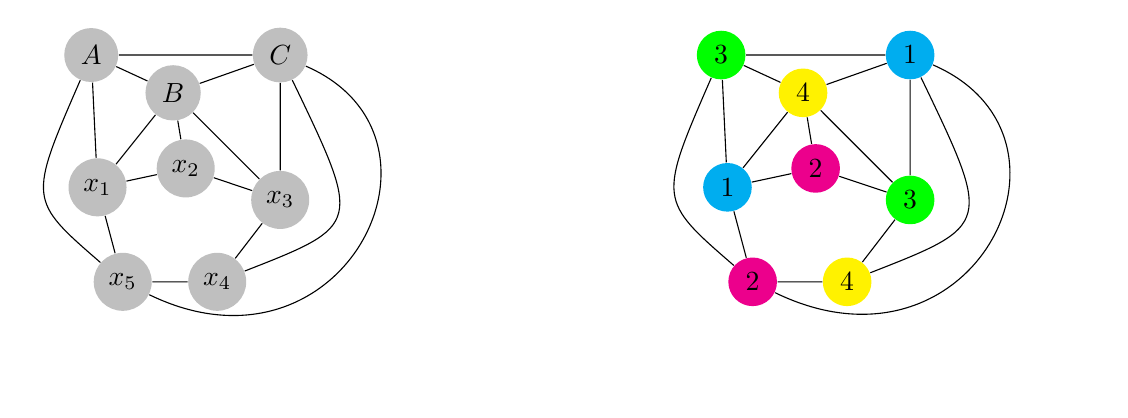
\begin{tikzpicture}
[scale=.8, auto=left, every node/.style={circle, fill=lightgray}]

\node (n1) at (2.1,4.2) {$x_1$};
\node (n2) at (3.5,4.5) {$x_2$};
\node (n3) at (5,4) {$x_3$};
\node (n4) at (4,2.7) {$x_4$};
\node (n5) at (2.5,2.7) {$x_5$};

\node (a) at (2, 6.3) {$A$};
\node (b) at (3.3, 5.7) {$B$};
\node (c) at (5, 6.3) {$C$};

 \foreach \from/\to in
 {n1/n2, n2/n3, n3/n4, n4/n5, n5/n1, a/b, a/n1, a/c, b/n1, b/n2, b/n3, b/c, c/n3}
  \draw (\from) -- (\to);

\draw (a) .. controls (1, 4) .. (n5);
\draw (c) .. controls (6.3, 3.6) .. (n4);
\draw (c) .. controls (8, 5) and (6, 1) .. (n5);


\node[circle, fill=cyan] (m1) at (12.1,4.2) {$1$};
\node[circle, fill=magenta] (m2) at (13.5,4.5) {$2$};
\node[circle, fill=green] (m3) at (15,4) {$3$};
\node[circle, fill=yellow] (m4) at (14,2.7) {$4$};
\node[circle, fill=magenta] (m5) at (12.5,2.7) {$2$};

\node[circle, fill=green] (a2) at (12, 6.3) {$3$};
\node[circle, fill=yellow] (b2) at (13.3, 5.7) {$4$};
\node[circle, fill=cyan] (c2) at (15, 6.3) {$1$};

 \foreach \from/\to in
 {m1/m2, m2/m3, m3/m4, m4/m5, m5/m1, a2/b2, a2/m1, a2/c2, b2/m1, b2/m2, b2/m3, b2/c2, c2/m3}
  \draw (\from) -- (\to);

\draw (a2) .. controls (11, 4) .. (m5);
\draw (c2) .. controls (16.3, 3.6) .. (m4);
\draw (c2) .. controls (18, 5) and (16, 1) .. (m5);
\end{tikzpicture}
\end{figure}
\label{pr:3:end}
Then after recoloring the graph as proposed, vertices $A$ and $B$ will both be colored with color $2$, which shows the new coloring is not proper. $\qed$

\section*{Problem 4}\label{pr:4:start}
(Bollab\'as, problem 5.36) Prove that if the graph $G$ has an orientation having no directed path with more than $k$ vertices, then $\chi(G) \leq k$.
\subsection*{Solution:}
\subsubsection*{Remark 1:}
We note that this result can actually be made an ``iff" statement.  That is to say, a graph $G$ has an orientation with no directed path having more than $k$ vertices iff $\chi(G) \leq k$.  To see the reverse direction, suppose we have a coloring $f : V(G) \to \{1, 2, \ldots, k\}$.  Then simply orient the edges to point in such a way that $f$ is stricly decreasing [this is possible because $f(x) = f(y)$ implies $x \not \sim y$].  In fact, this shows that [$\chi(G) \leq k$] implies [there's an \textit{acyclic} orientation with no long paths].  Thus, putting this together with the original claim, we obtain as an interesting corollary the following:
\begin{quotation}
There exists an orientation of $G$ without directed paths of more than $k$ vertices iff there exists such an orientation that's also acyclic.
\end{quotation}
Of course, if we had an independent proof of this assertion, we could prove the original claim quite quickly by viewing $G$ has a poset of height at most $k$.  Then the result is essentially Mirsky's theorem (the dual of Dilworth's theorem).

\subsubsection*{Remark 2:}
Remark 1 was the first thing I wrote for my solution.  Then I went to wikipedia to look for `height of a poset' to see what the convention was [if it's number of elements in longest chain or that plus/minus 1].  In doing so, I quickly hit the page for Mirsky's theorem, and it linked to the \textit{Gallai-Hasse-Roy-Vitaver theorem}, which is apparently precisely the result we are to prove in this problem.  I didn't look at the proof, but instead tried coming up with my own.  After my attempted proof got into some nested subcase and the notation became an absolute mess, I (in my frustration) peeked at wikipedia's proof.  I saw the phrase `maximal acyclic subgraph' and then stopped.  Below is the proof I made with this phrase in mind (which I ought to have thought of especially since I essentially said that in remark 1).

\subsubsection*{Solution:}
Let $G$ be a graph with an orientation having no directed path with more than $k$ vertices.  For this orientation, let $\sigma$ be a maximal acyclic subgraph (maximal with respect to edge set).  Then $\sigma$ gives rise to a partial ordering on the vertices of $G$.  That is, we say $a \geq_{\sigma} b$ iff there is a directed path in $\sigma$ from $a$ to $b$.  The fact that $\sigma$ is acyclic corresponds to the antisymmetry of this relation.
\paragraph*{}Since $G$ has no directed paths with more than $k$ vertices, and $\sigma$ is the induced orientation of a subgraph of $G$, it follows that $\sigma$ has no directed paths with more than $k$ vertices.  Therefore, in the poset corresponding to $\sigma$, the longest chain has at most $k$ vertices.  Let $A_1$ denote the set of $\sigma$-maximal elements of $V(G)$.  In general, for $i \geq 2$ let $A_i$ be the $\sigma$-maximal elements of $V(G) \setminus (A_1 \cup A_2 \cup \cdots \cup A_{i-1} )$, and iterate this until $A_1 \cup \cdots \cup A_t = V(G)$.  Since the longest $\sigma$-chain has at most $k$ vertices, we must have that $t \leq k$ (which is a common proof of Mirsky's theorem).
\paragraph*{}Each $A_i$ is a $\sigma$-antichain, so there are no $\sigma$-directed paths from vertices in any given $A_i$.  In fact, we claim that each $A_i$ is an independent set of $G$.  Having proven this, we will have exhibited a partition of $G$ into at most $k$ independent sets showing $\chi(G) \leq k$.
\paragraph*{}Suppose by way of contradiction that $x \neq y$ are in $A_i$ and $x \sim_{G} y$.  Without loss of generality, suppose the edge in the underlying orientation of $G$ is $x \to y$.  Now $x \to y$ is not in $\sigma$ since $A_i$ is a $\sigma$-antichain, which means by maximality of $\sigma$ that adding $x \to y$ to $\sigma$ would create a directed cycle.  Let $(a_1, a_2, \ldots, a_s)$ with $a_1 = x$ and $a_2 = y$ be this directed cycle.  Then all these directed edges except the initial $x \to y$ are in $\sigma$, which means means that we need $y >_{\sigma} a_3 >_{\sigma} a_4 >_{\sigma} \cdots >_{\sigma} a_s >_{\sigma} x$.  Therefore, by transitivity $y >_{\sigma} x$.  But this contradicts the fact that $A_i \supseteq \{x,y\}$ is a $\sigma$-antichain. $\qed$

\ignore{
\subsubsection*{Crappy attempt:}
We will prove this by induction on $k$.  If $k=0$ the claim is pleasantly trivial.  To assure our readers that this base case is valid we also remark that the claim for $k=1$ is almost more trivial (because it involves less thinking).  And because I'm a nice guy, a base case with any substance (though not much) is $k=2$.  For $k=2$, we can partition the vertices as sources and sinks.  There are no vertices with both edges coming in as well as edges coming out, and (clearly) the sources and sinks form independent sets in $G$.  Any isolated vertices of course can be colored arbitrarily.
\paragraph*{}For notational convenience, let $\Pee(k)$ be the property that a graph has an orientation without directed paths having more than $k$ vertices.  Suppose $G$ satisfies $\Pee(k)$.  If $G$ also satisfied $\Pee(k-1)$, then we would be done by induction.  So suppose $G$ has an orientation whose longest directed path has exactly $k$ vertices.  We will think of this orientation as fixed, and we will delete vertices progressively.  Subgraphs of $G$ inherit this orientation in the natural way.
\paragraph*{}Perform the following algorithm on $G$.
\texttt{
\begin{itemize}
\item[(0)] Initialize $i = 1$ and define $G_0 = G$.
\item[(1)] Define $v_i$ to be a vertex of $G_{i-1}$ such that there is a directed path\\in $G_{i-1}$ with $k$ vertices starting at $v_i$.
\item[(2)] Define $G_{i} = G_{i-1} \setminus \{v_i\}$.
\item[(3)] If there is a directed path of $k$ vertices in $G_{i}$, iterate $i$ and go to (1).
\end{itemize}
}
Suppose the algorithm terminates after $m$ iterations.  So we have vertices $\{v_1, \ldots , v_m\}$ and a graph $G_{m} = G \setminus \{v_1, \ldots , v_m\}$.  Then by design, when the algorithm terminates, $G_{m}$ will satisfy $\Pee(k-1)$, so by induction, it can be colored with $k-1$ colors.  We claim that $\{v_1, \ldots , v_m\}$ is an independent set of $G$, which would mean that the $(k-1)$-coloring of $G_m$ could be extended to a $k$ coloring of $G$ simply by giving all the vertices of the set $\{v_1, \ldots , v_m\}$ some new color.  This would complete the proof.
\paragraph*{}Suppose by way of contradiction that $v_i \sim_{G} v_j$ and $i < j$.  So we do not drown in indices, we will assume $i=1$ (this is actually just fine because of the self-similar nature of our algorithm).  The edge $ij=1j$ in the orientation of $G$ cannot go from $1$ to $j$.  If this were the case, then since there is a directed path in $G_{j-1} \not \ni v_1$ with $k$ vertices starting at $v_j$, then it could be extended by adding $v_1$ to the front [contradicting that $G$ satisfies $\Pee(k)$].  Therefore, the edge $1j$ must be oriented from $j$ to $1$.  But by the same logic, if $v_1 = a_1, a_2, \ldots , a_k$ is a directed path of $k$ vertices in $G_0$ starting at $v_1$, then we must have that $v_j \in \{a_2, \ldots , a_k\}$ or else we could add $v_j$ to the front of this path.
\paragraph*{}So it must be the case that $v_j = a_{l}$ for some $1 < l \leq k$.  Let $v_j = b_1, b_2, \ldots , b_k$ be the directed path in $G_{j-1}$ of $k$ vertices starting at $v_j$.

\paragraph*{}Wait!  Crap!  There's a graph for which this algorithm fails to produce an independent set.  :-/
}
\label{pr:4:end}


\section*{Problem 5}\label{pr:5:start}
Let $G$ be a triangle-free graph.
\begin{itemize}
\item[(a)] Prove that $\chi(G) \leq \sqrt{2 |V(G)|}$.
\item[(b)] For any graph $H$ and positive integer $d$, if $H$ has a subgraph of minimum degree at least $d$ then $\chi(H) \leq \max(d, \chi(H'))$, where $H'$ is any subgraph of $H$ that is maximal among subgraphs of $H$ of minimum degree at least $d$.  (Note that if $H$ itself has minimum degree at least $d$ then it is a triviality.)
\item[(c)] Prove $\chi(G) \leq \ceil{(4|E(G)|)^{1/3}}$.
\end{itemize}
\subsection*{Solution:}
\subsubsection*{Part a}
[I read the hint.  Honestly, I was barking up the right tree without it.] Following the hint, we will prove by induction on $k$ that if $|V(G)| < (k+1) ^2 / 2$ then $\chi(G) \leq k$, from which the desired bound follows immediately.  If $k=0$, then the claim is trivial.  If $k=1$, then $|V(G)| < 2$, in which case the claim is also trivial.  If $k=2$, then $|V(G)| < 4.5$, and since graphs with at most $4$ vertices are bipartite iff they are triangle-free the claim again follows.
\paragraph*{}Now suppose $k^2 / 2 \leq |V(G)| < (k+1)^2 / 2$, $G$ is triangle-free, and $k \geq 3$.  We can assume without loss of generality that $G$ is connected or else we could just apply our argument to each connected component.  Since $G$ is connected, triangle-free, and $k \geq 3$, it follows that $G$ is not a complete graph, and if $G$ is a cycle the claim follows trivially.
\paragraph*{}Thus, if the maximum degree of $G$ is less than or equal to $k$, then $\chi(G) \leq k$ by Brook's theorem.  Therefore, we can assume $x \in V(G)$ is a vertex of degree at least $k+1$.  Let $N(x)$ be the neighborhood of $x$, and let $H = G \setminus N(x)$.  Then since $|N(x)| \geq k+1$, it follows that $|V(H)| < (k+1)^2 / 2 - (k+1) = (k^2 + 2k +1) /2 -k-1 = k^2 / 2 - 1/2 < k^2 / 2$.  Therefore, by induction $H$ can be colored with at most $k-1$ colors.  And $N(x)$ must be an independent set since $G$ is triangle-free.  Therefore the coloring of $H$ can be extended to a coloring of $G$ simply by coloring $N(x)$ some new color. $\qed$

\subsubsection*{Part b}
Suppose there is a counter-example and let $H$, and $d$ be a graph and non-negative integer such that $(|V(H)|, d)$ is lexicographically minimal.  Then we need $|V(H)| > 1$, and we also need $d > \delta(H)$, where $\delta(H)$ is the minimum degree of $H$ or else the claim would in fact hold.  Since $H$ has a subgraph of minimum degree at least $d$ and $\delta(H) < d$, it follows that there is some vertex $v \in V(H)$ such $d(v) = \delta(H)$ and every subgraph of $H$ with minimum degree at least $d$ is necessarily a subgraph of $H \setminus \{v\}$.  Let $H' \subseteq H \setminus \{v\} \subseteq H$ be a subgraph of $H$ that is maximal with the property that $H'$ has minimum degre at least $d$.  By minimality of $(|V(H)|, d)$, since $H'$ is also maximal in $H \setminus \{v\}$, we have $\chi(H \setminus \{v\}) \leq \max(d, \chi(H'))$.
\paragraph*{}On the other hand, since $H$ is assumed to be a counter-example, we need $\chi(H) > \max(d, \chi(H'))$.  But we know $\chi(H) \leq \chi(H \setminus \{v\}) + 1$, so this implies
\[
\chi(H \setminus \{v\}) \leq \max(d, \chi(H')) < \chi(H \setminus \{v\}) + 1.
\]
Thus, $\chi(H \setminus \{v\}) = \max(d, \chi(H')) \geq d > \delta(H) = d(v)$.  But since $d(v) < \chi(H \setminus \{v\})$, we have $\chi(H \setminus \{v\}) = \chi(H)$, which is a contradiction. $\qed$

\subsubsection*{Part c}
If $\sqrt{2 |V(G)|} \leq \ceil{(4|E(G)|)^{1/3}}$, then we can simply apply part a.  Therefore, we can assume $\sqrt{2 |V(G)|} > \ceil{(4|E(G)|)^{1/3}}$, which implies $\sqrt{2 |V(G)|} > (4 |E(G)|)^{1/3}$, and thus
\[
|V(G)|^3 > 2 |E(G)|^2.
\]
\hrule
\paragraph*{}So I'm in beautiful southern California now.  It was one thing when I was working on this in the airplane and in my lay-over in Denver.  But I can literally see the Pacific Ocean and at least seventeen palm trees from where I'm sitting right now.  And besides, this is the only problem I didn't complete.  So I'm gonna hang up my hat and put my toes in the water (at least metaphorically).
\paragraph*{}Thus completing the proof. $\qed$

\label{pr:5:end}

\section*{Problem 6}\label{pr:6:start}
Problem takes forever to write.  It's the one about a game between builder and colorer.  Builder builds a graph on $[n]$ one vertex at a time, and colorer has to color it as they go along.  At the end, we'll have a graph, $G$.  The regret of the colorer is number of colors used divided by $\chi(G)$.  Builder's strategy will be as follows.
\paragraph*{}Let $k$ be the least integer such that $k 2^{k-1} \geq n$.  Builder is also constructing a table as he goes.  The table has $k$ columns, and one row for each color that colorer used so far.  Each entry of the table is a distinct vertex of the graph.  The builder will maintain that his table has the property (A) that vertices of color $r$ are all in row $r$, and (B) that vertices in the same column are independent.  The support of row $r$ (at time $j$) is $S_{j} (r) = S (r)$ is the columns corresponding to non-empty entries of row $r$.
\paragraph*{}On turn $j$, the builder's plan will be to find a subset $\emptyset \neq I \subseteq [k]$ such that $I$ is not equal to the support of any row.  He will then make a vertex $v_j$ and connect it to every vertex \textit{not} in a column contained in $I$.
\begin{itemize}
\item[(a)] Show that after colorer colors $v_{j}$, it is possible for builder to place $v_j$ in the table so as to maintain (A) and (B).
\item[(b)] Show that for every $j \leq n$, it is possible for builder to carry out the above strategy.
\item[(c)] Prove that if $n$ is sufficiently large, then the regret of colorer is at least $n/(\log_2 (n))^2$.
\end{itemize}
\subsection*{Solution:}
\subsubsection*{Part a}
Say $v_j$ is colored with color $r$.  Then clearly $S(r) \subseteq I$ or otherwise it would not be valid to color $v_j$ with that color.  Moreover, by the choice of $I$, we have $S(r) \neq I$.  Thus, $I \setminus S(r)$ is not empty.  We can then put $v_j$ in row $r$ and any column $c \in I \setminus S(r)$.  This spot will be empty, preserving property (A), and $v_j$ is not adjacent to anything in that column [since that column is contained in $I$], which preserves property (B). $\qed$

\subsubsection*{Part b}
Suppose by way of contradiction that on turn $j \leq n$, it is not possible to find such a set $I$.  Then for each set $\emptyset \neq I \subseteq [k]$, we must have some row whose support is equal to $I$.  Such a row would need $|I|$ elements in it.  Thus, the total number of elements in the table [which is equal to $j-1$] is bounded by
\[
n > j-1 \geq \sum_{\emptyset \neq I \subseteq [k]} |I| = \sum_{i=1}^{k} i \cho{k}{i} = k 2^{k-1},
\]
which contradicts the choice of $k$.  This last equality is easily proven by the following generatingfunctionological approach
\[
(1 + x)^{k} = \sum_{i=0} ^{k} x^{i} \cho{k}{i}, \qquad \qquad k (1+x)^{k-1} = \dfrac{d}{d x} (1 + x)^{k} = \dfrac{d}{dx} \sum_{i=0} ^{k} x^{i} \cho{k}{i} = \sum_{i=0} ^{k} i x^{i-1} \cho{k}{i}.
\]
The result then follows by specializing to $x=1$. $\qed$

\subsubsection*{Part c}
The number of colors used must be at least $n/k$ since each row of the table has at most $k$ non-empty entries, and at the end there are a total of $n$ such entries.  Furthermore, since the columns of the table are independent, this shows that $\chi(G) \leq k$.  Therefore, the regret satisfies
\[
regret \geq \dfrac{(n/k)}{k} = \dfrac{n}{k^2}.
\]
If $\log_2 (n) > 5$, we need to have $k \leq \log_2(n)$.  Otherwise, since $(k-1) 2^{k-2} \leq n$, we would have
\[
n \geq \dfrac{1}{4}[\log_2(n) -1] \times n > n,
\]
which would be a contradiction.  Now let $X= \{1, 2, 5, 6, 7, 13, 14, 15\}$.  Then a simple examination of cases with $n \leq 32$ shows that $k > \log_{2} (n)$ iff $n$ is in $X$.  Thus, for all $n \notin X$ [and in particular for all $n > 15$], the regret is at least $n/k^2 \geq n/(\log_2 (n))^2$, as desired. $\qed$

\label{pr:6:end}
\end{document}